\subsection{How to process data without a GUI}

\begin{frame}
	How to process data without a GUI.
\end{frame}

\begin{frame}
	\frametitle{Data Science at the Command Line\cite{janssens2021}}
	\begin{columns}
		\begin{column}{0.5\textwidth}
			\begin{itemize}
				\item Get data from websites, APIs, databases, and
				      spreadsheets; scrub text, CSV, HTML, XML, JSON.
				\item Explore data, compute statistics, create
				      visualizations.
				      %\item Manage your data science workflow.
				\item Create your own tools, re-use code.
				\item Parallelize and distribute data pipelines.
				\item Model data with dimensionality reduction, regression, and
				      classification algorithms.
				\item Command line from Python, Jupyter, R, RStudio, Apache
				      Spark.
				\item Read online~\href{https://jeroenjanssens.com/dsatcl}
				      {here}.
			\end{itemize}
		\end{column}
		\begin{column}{0.5\textwidth}
			\begin{figure}
				\centering
				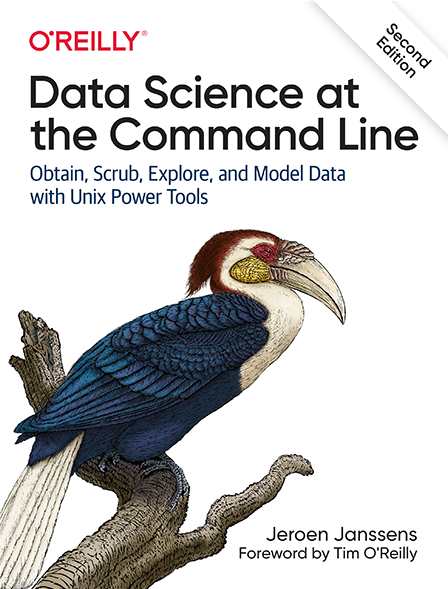
\includegraphics[scale=0.3]
				{img/data_science_at_the_command_line.png}
			\end{figure}
		\end{column}
	\end{columns}
\end{frame}

\begin{frame}
	\frametitle{GRASS GIS}
	\begin{columns}
		\begin{column}{0.5\textwidth}
			\begin{itemize}
				\item Geographic Resources Analysis Support System.
				\item Vector and raster geospatial data management,
				      geoprocessing, spatial modelling, and visualization.
				\item Free, Libre, and Open Source Software.
				\item Docker container.
				\item Open Source GIS: A GRASS GIS Approach~\cite{neteler2008}.
			\end{itemize}
		\end{column}
		\begin{column}{0.5\textwidth}
			\begin{figure}
				\centering
				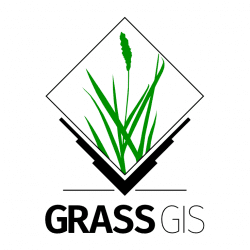
\includegraphics[scale=0.5]{logos/grassgis.png}
			\end{figure}
		\end{column}
	\end{columns}
\end{frame}

\begin{frame}
	\frametitle{Orfeo ToolBox (OTB)}
	\begin{columns}
		\begin{column}{0.5\textwidth}
			\begin{itemize}
				\item OTB is a set of state-of-the-art remote sensing tools.
				\item It is FOSS (Free Open Source Software).
				\item Wide variety of applications available: from
				      ortho-rectification or pansharpening, all the way to
				      classification, SAR processing, and much more!
				\item \url{www.orfeo-toolbox.org}
			\end{itemize}
		\end{column}
		\begin{column}{0.5\textwidth}
			\begin{figure}
				\centering
				
\includegraphics[scale=0.8]{logos/orfeo-toolbox.png}
			\end{figure}
		\end{column}
	\end{columns}
\end{frame}

\begin{frame}
	\frametitle{GDAL programs/utilities}
	\begin{columns}
		\begin{column}{0.5\textwidth}
			\begin{itemize}
				\item GDAL is a translator FOSS library for raster and vector
				      geospatial data.
				\item It presents a single raster abstract data model and
				      single vector abstract data model to the calling
				      application for all supported formats.
				\item It also comes with a variety of useful command line
				      utilities for data translation and processing.
				\item Docker container.
				\item \footnotesize{\url{https://gdal.org/programs/index.html}}
				\item \href{https://spatialthoughts.com/courses/mastering-gdal-tools/}{Mastering GDAL tools}.
			\end{itemize}
		\end{column}
		\begin{column}{0.5\textwidth}
			\begin{figure}
				\centering
				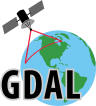
\includegraphics[scale=0.2]{logos/gdalicon.png}
			\end{figure}
		\end{column}
	\end{columns}
\end{frame}
